% This is samplepaper.tex, a sample chapter demonstrating the
% LLNCS macro package for Springer Computer Science proceedings;
% Version 2.20 of 2017/10/04
%
\documentclass[runningheads]{llncs}
%
\usepackage{graphicx}
\usepackage{xcolor}
\usepackage{multicol}
\usepackage{float}
\usepackage{wrapfig}
\usepackage{textcomp}
% Used for displaying a sample figure. If possible, figure files should
% be included in EPS format.
%
% If you use the hyperref package, please uncomment the following line
% to display URLs in blue roman font according to Springer's eBook style:
% \renewcommand\UrlFont{\color{blue}\rmfamily}

\begin{document}
%
\title{Open OnDemand: HPC for everyone\thanks{Supported by National Science Foundation grant 1835725.}}
%
%\titlerunning{Abbreviated paper title}
% If the paper title is too long for the running head, you can set
% an abbreviated paper title here
%
\author{Robert Settlage\inst{1}\orcidID{0000-0002-1354-7609} \and
Alan Chalker\inst{2}\orcidID{0000-0002-5475-8779} \and
Eric Franz\inst{2} \and
Steve Gallo\inst{3}\orcidID{0000-0002-4854-9858} \and
Edgar Moore\inst{1}\orcidID{0000-0002-3229-8249} \and
David Hudak\inst{2}\orcidID{0000-0002-9043-0850}}
%
\authorrunning{R. Settlage et al.}
% First names are abbreviated in the running head.
% If there are more than two authors, 'et al.' is used.
%
\institute{Advanced Research Computing, Virginia Tech, Blacksburg VA 24060, USA \and
Ohio Supercomputer Center, Columbus OH 43212, USA \and
Center for Computational Research, University of Buffalo, Buffalo NY 14203, USA\\
\email{rsettlag@vt.edu}}
%
\maketitle              % typeset the header of the contribution
%
\begin{abstract}
Open OnDemand is an open source project designed to lower the barrier to HPC use across many diverse disciplines.  Here we describe the main features of the platform, give several use cases of Open OnDemand and discuss how we measure success.  We end the paper with a discussion of the future project roadmap.

\keywords{Open OnDemand \and Science Gateways \and high performance computing \and interactive \and HPC.}
\end{abstract}
%
%
%
\section{Introduction}
In today\textquotesingle s world, where we are producing, monitoring and making decisions based on many zettabytes of data daily, access to computing is of paramount importance\cite{ref_proc1} .  To make sense of all of this data, many scientists rely on high performance computing (HPC) clusters.  These clusters have been the workhorse in many domains such as engineering, physics, computational chemistry, and geosciences.  Unfortunately, access to these computational tools is generally not through familiar web-based tools, but instead most frequently access is through a Secure Shell (SSH), requires familiarity with Linux and command-line, and file transfer tools (FTP) etc which, when taken in aggregate, has introduced a barrier to access of the computational power available in these HPC clusters.  This accessibility gap is a long standing and recognized issue in HPC.  Reducing, or ideally removing, this barrier will lead to immediate improvements in cluster accessibility and productivity across a wide range of data intensive disciplines.  

Open OnDemand\cite{ref_article1} is an innovative, open-source, web-based portal for accessing HPC services that removes these intricacies.  By providing more familiar web-based access to the HPC clusters, not only does Open OnDemand reduce the barrier to use, it has also been shown to reduce the time to science.  In fact, the median time from initial login to first job submission for all new OSC clients in 2017 using OnDemand was 10 times faster than those using traditional access methods.  Through OnDemand, HPC users can upload and download files, create, edit, submit and monitor jobs, create and share apps, run GUI applications and connect to a terminal, all via a web browser, with no client software to install and configure. OnDemand greatly simplifies access to HPC resources, freeing disciplinary scientists from having to worry about the operating environment and instead focus on their research.  In this paper, we will focus on:
\begin{enumerate}
    \item Open OnDemand features highlighting ease-of-use,
    \item Examples and use cases,
    \item Success stories,
    \item Future work, i.e. the roadmap.
\end{enumerate}

\section{Features -- Ease of Use}

Open OnDemand is a web-based portal of entry to HPC clusters with a primary goal of lowering the barrier to use of the computational power and tools within the cluster.  Open OnDemand provides a rich set of core web applications which leverage HTML5 standards and are securely hosted behind a web proxy providing federated authentication. All the user needs to access OnDemand is a modern web browser and their HPC credentials. OnDemand provides HPC centers a “zero-install” (i.e. no native SSH, SFTP, or VNC client necessary) and single sign-on (SSO) solution for their users.  

In an Open OnDemand enabled HPC center, a user can access the clusters by using command line SSH or by browsing to the OnDemand URL hosted by the HPC center and authenticating with their HPC credentials. Thus, Open OnDemand does not replace traditional access but rather provides another avenue to gain access.  Upon authentication, the user is presented with the Dashboard App which serves as the landing page for OnDemand and enables discovery of the various OnDemand apps, Figure  \ref{fig-dshapp}.  Note the Dashboard App allows for HPC center branding and news/message of day display (left Figure \ref{fig-dshapp}).  A default installation of OnDemand includes the following core apps: File Explorer and File Editor for file management, Active Jobs and Job Composer for job management and monitoring, as well as a Shell App for command line access.  Note that OnDemand allows a single portal to several clusters within the HPC center.  For instance, at Virginia Tech, we currently have an IBM Power8 and two X86 clusters served by a single OnDemand portal.

\begin{figure}[H]
\centering
\includegraphics[width=0.475\textwidth]{figures/dashboard-v3.eps}
\hfill % <-- Seperation
\includegraphics[width=0.475\textwidth]{figures/vt-ood-page.eps}
\caption{On the left, the Dashboard app landing page showing branding and message of day.  On the right, an example of the app landing page showing users the current apps installed at VT. } \label{fig-dshapp}
\end{figure}

In this basic installation, Open OnDemand has simplified the user experience by giving users a more familiar web portal to the HPC systems and simple tools to transfer files to/from the system and finally both a text editor and job composer.  These basic tools are all web based and allow users to skip the command line to move files, edit scripts and submit job requests all via the web portal.  

The basic functionality described above is really the launching point for center and user customization.  HPC Centers can tailor the application set to those found most used or that cause the most tickets to create a highly customized installation.  Open OnDemand supports web applications written in a variety of languages including Ruby, Python and Node.js and allows for creating custom user applications.  These can, for instance, be used to make portals for interactive apps such as Jupyter Notebooks, Rstudio, Matlab, ParaView, Comsol, etc (see Figure \ref{fig-dshapp} right for example).  Similarly, users can create modifications to the standard (or Center) installed set of applications to create tools more suitable to their individual workflows.  To further enable this, the Dashboard comes with a plug-in style wrapper to stream-line the App development process.  Not only can users edit and create custom apps, they can share these new apps with other users.  Through this extensibility mechanism, we envision OnDemand capable of remaining a relevant tool to enabling use of HPC resources across many disciplines today and in the future.  

\section{Example Apps and Use Cases}

At this point, Open OnDemand has a diverse user base and has seen many successes.  Below we highlight three important applications, two are standard upon installation of Open OnDemand while the third is an Interactive App showing the extensibility of the platform.

\newpage

\subsection{Files App}

\begin{wrapfigure}{r}{0.5\textwidth}
    \includegraphics[width=0.48\textwidth]{figures/file-access-v3.eps}
    \caption{The Files App gives users a web-based look at HPC storage allowing them to manage files in a familiar environment.} \label{fig-filesapp}
\end{wrapfigure}

The Files App is perhaps the most important example of how presenting users with familiar tools can lower the barrier to use of HPC clusters.  Traditional command line access via SSH requires file management from a terminal.  While users familiar with Linux are used to the raw and powerful file editing and transfer tools such as vim, ftp, scp and rsync, for new users, this is often a formidable barrier.  The Files App (Figure \ref{fig-filesapp}) provides another avenue to create files and folders, view files, manipulate file locations, upload and download files all in the familiar tree view users are accustomed to using on their local system.  Providing this file management interface both reduces the anxiety of new users and reduces inadvertent learning errors (e.g. \textit{rm -rf}).

\subsection{Job Composer}

The most important aspect of working in an HPC environment is navigating the complexities of submitting compute tasks as a job to a resource scheduler such as PBS, LSF or Slurm. Indeed, interacting with resource schedulers is an often daunting, confusing and yet necessary component of working on shared HPC systems.  To facilitate the use of schedulers, Open OnDemand has an application, the Job Composer, which provides a web-based utility for creating and managing batch jobs from template directories (Figure \ref{fig-jobapp}). The Job Composer App attempts to model a simple but common workflow typical of users in HPC centers. When users create new batch jobs they often:

\begin{enumerate}
    \item Copy a directory of a previous job, either one of their previous jobs or a job from a group member
    \item Make minor modifications to the input files
    \item Submit this new job
\end{enumerate}

\noindent Through the Job Composer, users can create new jobs based on previous jobs (templates), create new job templates, view status of jobs, view results and more.  By abstracting away the command line to facilitate this workflow, the Job Composer again allows use of familiar tools to accomplish HPC tasks such as job creation, scheduling and deletion.

\begin{figure}[H]
\centering 
\includegraphics[width=0.75\textwidth]{figures/job-constructor-v3.eps}
\caption{The Job Composer App provides a template based abstraction to submit jobs to HPC schedulers.} \label{fig-jobapp}
\end{figure}

\subsection{Jupyter Notebooks}

Much of science is accomplished through interactive GUI based applications, if not for the full compute, for prototyping, troubleshooting, experimenting and creating figures.  A hallmark of Open OnDemand is that not only does it \textit{allow} interactive applications, it \textit{facilitates} their use through providing a mechanism to abstract the environment setup and gives users a mechanism to connect to the running application (often a weblink).  In the case of Jupyter Notebooks, OnDemand creates a batch job, configures the environment and gives the user a clickable weblink to the running Jupyter Notebook (Figure \ref{fig-jnapp}).  Due to the demand for interactive GUI applications such as Jupyter Notebooks, Matlab, Rstudio, Comsol etc, the Dashboard comes with a plug-in style wrapper designed to streamline App development.  Importantly, sites can develop site specific apps for distribution to their users.

\begin{figure}[H]
\centering
\includegraphics[width=0.475\textwidth]{figures/jn-launch.eps}
\hfill % <-- Seperation
\includegraphics[width=0.475\textwidth]{figures/jn-ex.eps}
\caption{Interactive App page showing status of a Jupyter Notebook job (left).  The link sends the user to the running Jupyter Notebook (right).} \label{fig-jnapp}
\end{figure}


\section{Successes}

\subsection{VT OpenPOWER Hackathon}

In Spring 2019, VT hosted an OpenPOWER Hackathon.  The goal of the hackathon was to expose users to the acceleration possible when using the PowerAI framework on an IBM Power8 cluster.  Many of the participants were new HPC users but had significant experience with creating Deep Learning applications on local hardware.  Often, new HPC cluster users, even those familiar with Linux, experience some amount of time lag between account creation and first successful job.  In a limited time hackathon, this added overhead distracts from the goal of the hackathon by shifting the focus from the hackathon topic to learning HPC idiosyncrasies.  By utilizing the Open OnDemand web portal, we were able to successfully launch the hackathon with no user setup and had users computing in Jupyter Notebooks as soon as they typed in the web address.  Further, we were able to create an OnDemand App with the PowerAI environment preloaded as a conda environment.  The conda environment included all the PowerAI optimized tools including TensorFlow, mpi, ddlrun etc.  For those users that took advantage of the Open OnDemand interface, we had zero issues and very little time was required to get these users into a computing environment such that we had more time to discuss the hackathon topics and less time was devoted to troubleshooting user environment issues.  As an added benefit, some users were interested in using TensorBoard to view the neural networks they were creating to troubleshoot, monitor performance, etc.  Typically, this is an added complexity many users struggle with.  Of course, users familiar with creating SSH tunnels and using port forwarding are fully capable of setting up the environment and starting a TensorBoard.  However, our observation is even more sophisticated users choose to use the OnDemand app when available so that they can focus on the compute task rather than environment setup.


\subsection{Using HPC in the Classroom}

Similar to the issues faced in a limited duration hackathon, introducing students to HPC in a classroom setting can be daunting if the students are new to the command line, unfamiliar with SSH, and likely new to Linux.  OnDemand simplifies this introduction by abstracting away the initial SSH via the Shell App and unifies the user experience by providing a single portal to gain access to the HPC compute.  At VT, we have seen a dramatic decrease in the initial time to get students on our local HPC clusters.  What was taking 45 min of an hour lecture, making sure all the students had the proper tools installed (Putty, Terminal, etc) and logged in via 2-factor authentication, now takes less than 15 min and frees the instructor from troubleshooting local student platform issues allowing the focus to quickly return to the domain topic the instructor had planned.  Improving this initial experience is often critical in keeping the attention and participation within a classroom setting.  Even if the instructor simply uses OnDemand as the portal to the Shell App, we see an improved experience from two features: 1) all clusters enabled in the OnDemand installation are available in a pull-down menu (Figure \ref{fig-shellapp}) and 2) in our 2-factor environment, users are fully authenticated in the browser such that the Shell App is running as user.  It is our observation that this simple change, moving from multiple platform based shell access tools, to a single web-based shell tool is the single largest momentum changer when instructors are choosing local vs cloud resources for compute intensive courses.

\begin{figure}[H]
\centering
\includegraphics[width=0.475\textwidth]{figures/vt-clusters.eps}
\hfill % <-- Seperation
\includegraphics[width=0.475\textwidth]{figures/shell-v3.eps}
\caption{Left: The Dashboard app landing page showing the shell app pulldown allowing users to select target cluster. Right: A running shell.} \label{fig-shellapp}
\end{figure}

\section{Future Work}

In 2018, OSC with partners from Virginia Tech and SUNY Buffalo were awarded an NSF grant under the CSSI program managed by the Office of Advanced Cyber-infrastructure This ~\$3.3M award (\#1835725) provides funding through the end of 2023 and is formally titled “Frameworks: Software NSCI-Open OnDemand 2.0: Advancing Accessibility and Scalability for Computational Science through Leveraged Software Cyberinfrastructure” This new project combines two widely used HPC resources:

\begin{itemize}
    \item Open OnDemand 1.0 - an existing open-source, web-based project for accessing HPC services; and
    \item Open XDMoD - an open-source tool that facilitates the management of HPC resources.
\end{itemize}

\noindent with the following objectives:

\begin{enumerate}
    \item Visibility: Leverage XDMoD seamlessly from OnDemand, creating a unified platform for scientists to work with and optimize their HPC work.  
    \item Accessibility: Improve the OnDemand interface for more scientists \& fields of science.  
    \item Scalability: Extend the scalability of OnDemand for more platforms and applications.  
    \item Engagement: Conduct a program to engage departmental, campus and national HPC users along with the Science Gateway community to drive adoption and follow-on development.
\end{enumerate}

\noindent Here we highlight three aspects of the current efforts.

\subsection{Montitoring}

Monitoring system health and job performance is an important aspect of operating and using high performance computing clusters.  The overall system health and status of a cluster is useful on many levels but from a users perspective is often an indicator of where (what queue or cluster) they should submit new jobs.  Through the Open OnDemand dashboard, HPC administrators currently have the ability to give system status messages (Message of Day).  While this can alert users to quality of service issues, more granular and informative statistics as provided by XDMoD are often desirable. Efforts are currently underway to provide a mechanism for integration of XDMoD into Open OnDemand.  A prototype is shown in Figure \ref{fig-xdmod}.
Through this integration project, OnDemand users will be able to explore HPC resource availability at their local center.  By exposing this data to the users, they will have the information available to choose systems based on shorter queue time, higher availability of resources, quality of service, or other metrics they find useful.  
At OSC, Ganglia graphs providing static views of high level compute job resource utilization statistics have been integrated into job summaries.  Through this integration project, we will expose users to the additional functionality offered by XDMoD.  XDMoD allows users to view detailed performance information on their individual jobs and drill down to gain additional insights into how a job has performed including utilization of individual cores, filesystem throughput, and network activity over the course of the job.  By providing this easily accessible and usable view into job performance, we anticipate both experienced and novice users alike will identify aspects of their computations to optimize and improve.

\begin{figure}[H]
\centering
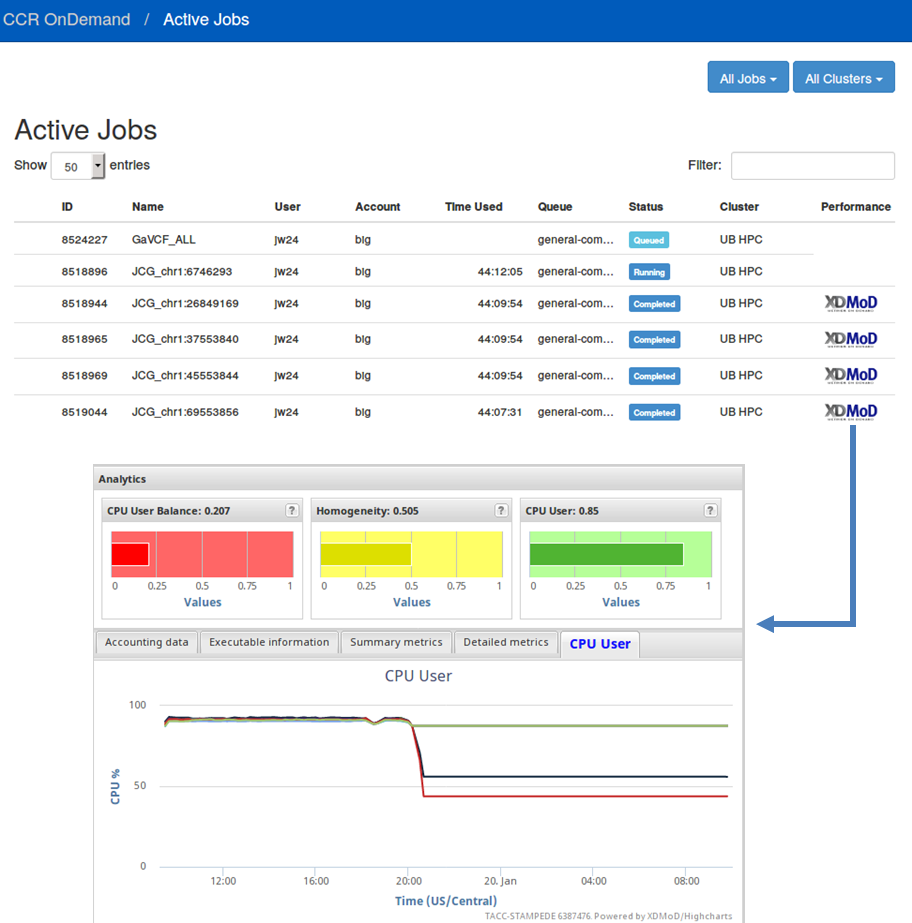
\includegraphics[width=0.475\textwidth]{figures/jobperformance.png}
\hfill % <-- Seperation
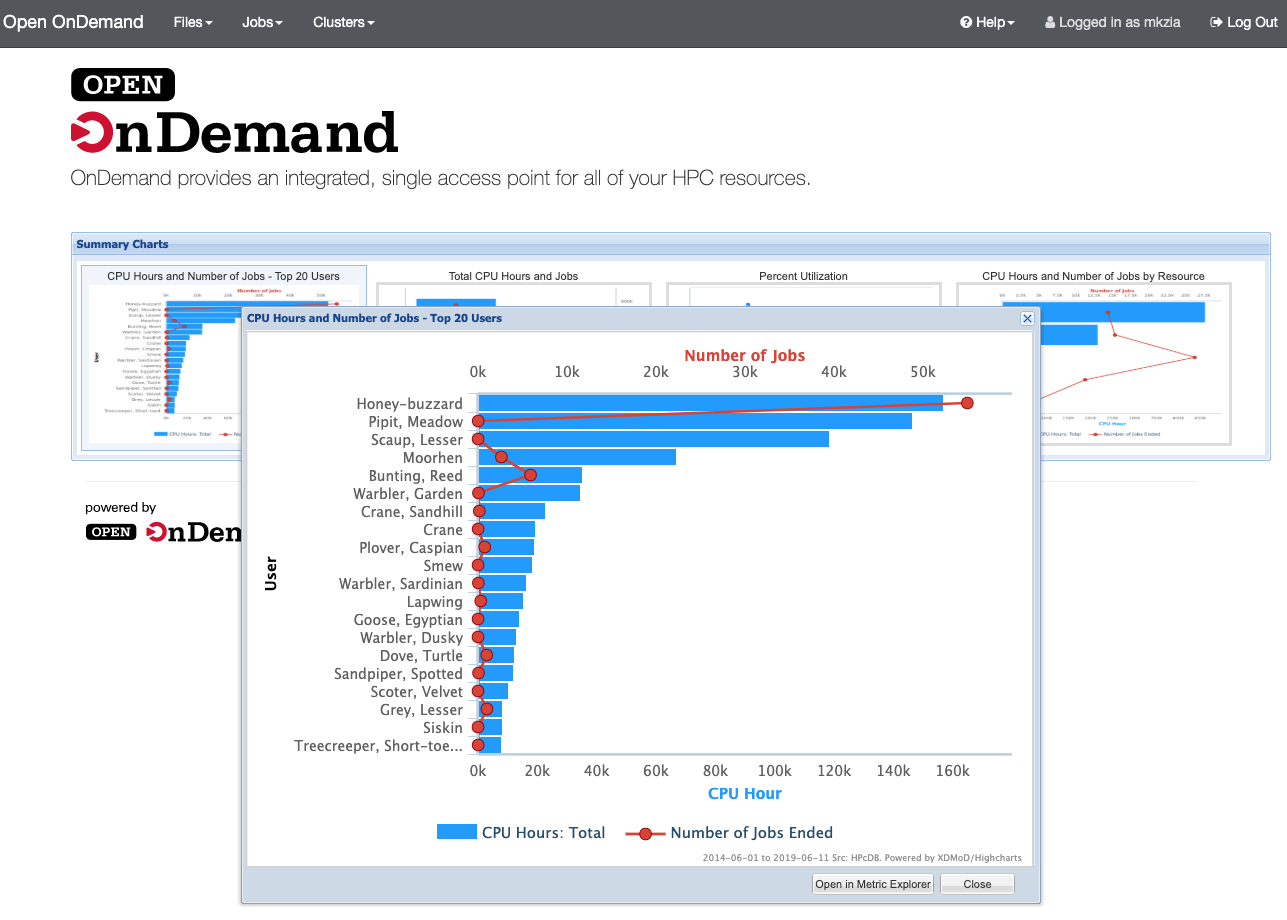
\includegraphics[width=0.475\textwidth]{figures/xdmod-dashboard-mock2.eps}
\caption{On the left, completed jobs showing XDMoD links for exploration of job performance.  On the right, the prototype XDMoD dashboard in Open OnDemand. Clicking on any chart displays an expanded view and allows the user to also view the chart directly in XDMoD for additional functionality. } \label{fig-xdmod}
\end{figure}

\subsection{Accessibility and Scalability}

Open OnDemand has an overarching goal of presenting HPC in a way that makes the computing resources more accessible to more users.  We see this as a challenge to both enable less sophisticated users and enhance the veteran power user.  For the less sophisticated user, as discussed above, the first step in accessibility is providing the user with more familiar tools to access the resources, i.e. web-based file management, job management and file editors.  As we move forward with these users, we envision we will need to further simplify the job execution phases of HPC use.  This could come in the form of a) tailoring some functionality towards a specific user base and b) providing more available apps spanning more fields of science.  In many cases, job execution could be completely automated and the functionality pushed from the users local desktop.  For these situations, we envision creation of a "desktop metaphore".  In our vision, a user could have an icon on their local computing device with the built in functionality to transfer data, submit a job to computing queue, and notify the user of successful completion of the compute job.  In a simple example, a user may drag and drop a Matlab file on a Matlab icon preconfigured to send the file and start the simulation on the local cluster.

Many data science and computing fields have been emphasizing repeatability and reproducibility.  To facilitate this, we will enable git functionality within the Job Composer to allow users to automatically commit job scripts into a code repository.  This will serve two purposes.  First, users will have an offline copy of their working scripts.  Second, in team settings, code repositories are an oft used method of collaboration.  While much of our effort has been lowering the barrier for novice users, we are looking for ways to enhance the productivity of all users.  For advanced users, we are working to enable parameter sweeps, job arrays and more advanced multi-step pipelines.  

While the Files App in it current form is transformative for many users and use cases, we do see some need for further enhancements.  Specifically, there is a need to support both larger file transfers and directory transfers.  Both have been problematic for similar reasons, namely speed of transfer and length of user attention span.  As a user moves their attention from the current task which is queued waiting for file(s) upload, the tendency is to forget the process is in-flight and inadvertently the system is shutdown, laptop lid closed, etc.  These are solvable issues and simply need some development time.

Cloud computing is an important computing platform that is complementary to traditional HPC clusters.  Some compute jobs/duties are better suited to a cloud environment but are still an important part of computing workloads.  Examples include running webservers as data collection devices, web based portals to submit data queries that may spawn HPC jobs, support of multiple operating systems for specialty software, etc.  In our view, cloud is simply another tool in a computing environment that enables our researchers.  As such, supporting spawning of virtual machines (VMs) in a cloud system should be another app in Open OnDemand.  Work is currently underway to extend the OnDemand apps to include native spawning of VMs though calls to an on-prem OpenStack installation at Virginia Tech.  This work will also be extended to provisioning VMs on public cloud systems as well.

\subsection{Engagement}

As with any software development project, success is an iterative milestone.  As this is community software, our users need to specify the milestones and give the measure of success.  Key to any community project is engagement and outreach to keep the project focused on user needs.  To keep Open OnDemand relevant to the community, we need to engage the community of users continuously to stay abreast of the state of the art codes and processing methods.  As the community develops, OnDemand must follow.  Today, web-based portals are the familiar interface users are looking for.  Perhaps the next wave will be towards mobile device applets.  To ensure we are connected to the community, we have formed an Advisory Group with representatives from many institutions spanning academia and industry.  This group meets at least Quarterly and discusses topics relevant to Open OnDemand usefulness, adoption, design, code sharing etc.  Our current schedule has us meeting at PEARC and Supercomputing with more frequent user meetings.  


%
% ---- Bibliography ----
%
% BibTeX users should specify bibliography style 'splncs04'.
% References will then be sorted and formatted in the correct style.
%
% \bibliographystyle{splncs04}
% \bibliography{mybibliography}
%
\begin{thebibliography}{8}

\bibitem{ref_proc1}
Reinsel, D., Grantz, J., and Rydning, J.: The Digitization of the World -- From Edge to Core. IDC White Paper – \#US44413318 (2018).

\bibitem{ref_article1}
Hudak, D., Johnson, D., Chalker, A., Nicklas, J., Franz, E., Dockendorf, T. and McMichael, B.L.: Open OnDemand A web-based client portal for HPC centers. Journal of Open Source Software. \textbf{3}(25), 622 (2018). \doi{10.21105/joss.00622}
\end{thebibliography}
\end{document}
